\documentclass[12pt]{article}

\usepackage{amsmath,amssymb,amsthm}
\usepackage{graphicx}
\usepackage{graphics}
\usepackage{enumerate}
\usepackage{caption}
\usepackage{subcaption}
\usepackage{multicol}
\usepackage{xcolor}
\usepackage{hyperref}

\begin{document}
	
	\sffamily
	\begin{center}
		\textbf{\Large{Math 120 - Problem Set - Chapter 0}} \\
\Large{Aidan Fraser (adf395)} %%% <---- Enter your name and NetID here.

	\end{center}

There are seven typos in the four mathematical expressions below. Edit the \LaTeX\ code below and compile to match those expressions in the boxed figure. You are not expected to understand any of the notation at this point in the course. The purpose of these exercises is to simply practice working with \LaTeX.

\begin{figure}[h]
    \centering
    \caption{Desired mathematical expressions} \label{fig:soln}
    \fbox{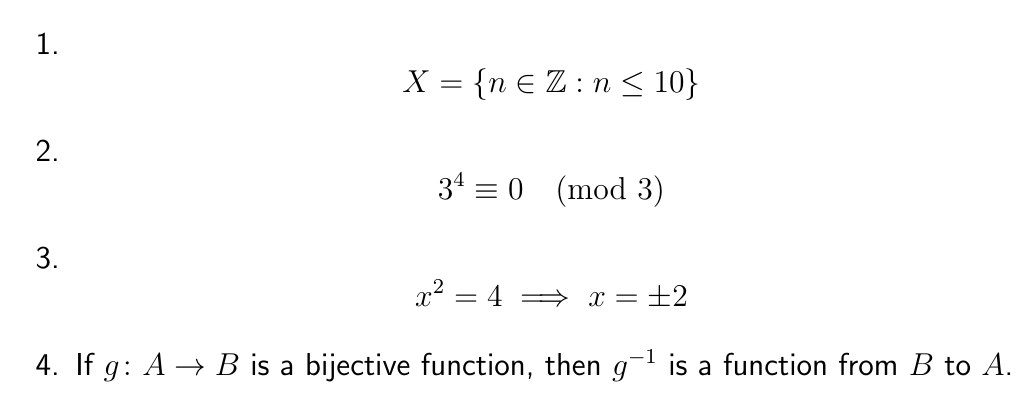
\includegraphics[width=6in]{solns.PNG}}
\end{figure}

%%% Edit the expressions below.
\begin{enumerate}
\item \[X = \{n \in \mathbb{Z} : n \le 10 \}\]

\item $$ 3^{4} \equiv 0 \pmod{3} $$

\item \[x^2 = 4 \implies x = \pm2\]

\item If $g\colon A \to B$ is a bijective function, then $g^{-1}$ is a function from $B$ to $A$.

\end{enumerate}

\end{document}

